\documentclass[]{aa}

\usepackage{txfonts}
\usepackage[colorlinks, breaklinks]{hyperref}
\usepackage{graphicx}
\graphicspath{{Article_figures/}{General_figures/}}
\hypersetup{linkcolor=blue, citecolor=blue, filecolor=black, urlcolor=blue}

\newcommand{\orcid}[1]{
\href{https://orcid.org/#1}{

\includegraphics[height=11pt]{ORCIDiD_icon128x128.png}}}

\newcommand{\prob}[2]{\mathcal{P}\left( #1 \mid #2\right)}

\begin{document}

\title{Implementation of the redshift evolution of type Ia supernovae in
SNANA}

\titlerunning{Implementation of the redshift evolution of type Ia supernovae in
SNANA}
\authorrunning{N.~Nicolas et al.}

\author{
    N. Nicolas \thanks{n.nicolas@ip2i.in2p3.fr, equal contribution} \inst{1} 
    \and M. Rigault \thanks{m.rigault@ip2i.in2p3.fr, equal contribution} \inst{1}
    \orcid{0000-0002-8121-2560}
    \and\\ Y. Copin \inst{1}
    \orcid{0000-0002-5317-7518}
    \and R. Graziani \inst{2}
    \and G. Aldering\inst{3}
    \and M. Briday\inst{1}
    \and Y.-L. Kim\inst{1}
    \orcid{0000-0002-1031-0796}
    \and J. Nordin\inst{4}
    \and Saul Perlmutter\inst{3}
    \and M. Smith\inst{1,5}
    \orcid{0000-0002-3321-1432}
}

\institute{Univ Lyon, Univ Claude Bernard Lyon 1, CNRS, IP2I Lyon / IN2P3, IMR
    5822, F-69622, Villeurbanne, France
    \and 
    Université Clermont Auvergne, CNRS/IN2P3, Laboratoire de
    Physique de Clermont, F-63000 Clermont-Ferrand, France
    \and
    Physics Division, Lawrence Berkeley National Laboratory, 
    1 Cyclotron Road, Berkeley, CA, 94720, USA
    \and
    Institut fur Physik, Humboldt-Universität zu Berlin, Newtonstr. 15,
    12489 Berlin, Germany
    \and
    University of Southampton, Southampton, UK
}

\date{Submitted to A\&A\ the 19th of May 2020 / Accepted 26 February 2021}

\abstract{The use of Type Ia supernovae (SNe~Ia) as standard candles lead to a
huge improvement on the constraints on cosmological parameters. In order to
continue refining these values in a era of increasingly bigger datasets,
systematic uncertainties have to be dealt with. Following previous work on the
link between supernovae and their environment, we aim at finding the precise
impact of a redshift-evolving underlying stretch distribution of SNe~Ia compared
to the currently-used distributions in SNANA.}

\keywords{Cosmology -- Type Ia Supernova -- Systematic uncertainties}
\maketitle

\section{Introduction}
\textit{General talk about SNe Ia, Hubble diagram, constraints and assumptions
from BBC to fit HD.}

Standardizing SNe Ia led to the discovery of the acceleration of the Universe's
expansion: thanks to their color and stretch parameters, the systematic
uncertainty on their absolute magnitude and thus their distance was greatly
reduced. Dark energy is commonly thought to be the cause of this expansion, and
its equation-of-state parameter, $w$, is currently know down to $\approx$ 4\% by
combining constraints from both SNe Ia and the Cosmic Microwave Background. If
we want to enhance that knowledge, apart from the statistical part it's the
systematic budget that needs to go lower.

With that goal in mind, some recent studies try to improve the known
correlations. In NR21, we presented an initial study of the drift of the
underlying SNe~Ia stretch distribution as the function of redshift. We based
this study on the assumption of two populations of SNe~Ia, young and old, and
implemented different modelings of their distributions to better represent the
observed data. For that end we took SNe~Ia data and created a complete sample by
applying redshift cuts corresponding to the expected distance where no selection
effects should impact each survey. This approach was at the time the
simplest one to implement but does not allow to ponder the impact such a
modeling has on the cosmology, and mainly on $w$, and skips all selection
effects altogether.

Other studies tend to define and refine other correlations between a SN's
brightness and some observable properties, such as their host-galaxy's mass or
Star Formation Rate. One of the most common ways to test these correlations is
to simulate surveys by using underlying distributions of parameters and
correlations between them with the aim to find which ones come closest to the
actual data. In the SNANA framework, it's a galaxy's stellar mass
($M_\mathrm{stellar}$) that is assumed as the main observable responsible for
its environmental effects on SNe Ia. Selection effects are simulated for each
survey with great accuracy, and the goal is to correct the values of SNe
affected by Malmquist bias by computing the average

\section{Modeling}\label{sec:model}
In our previous work N21, we had determined a relationship between SNe~Ia
stretches and redshift by using the evolution of the fraction of young SNe~Ia,
$\delta(z)$, after having modelized each sub-population's underlying stretch
populations based on LsSFR, a tracer for the age of a supernova.

In order to simulate SNe, we require a host galaxy to follow the distributions
of what has been observed by different surveys. While we argue that LsSFR is a
better tracer of a SNe's environment (Briday 21), most survey characterize
galaxies using their stellar mass. Therefore, to compare the implication of our
modeling based on LsSFR with what other surveys observed, we need to modelize
galaxy masses with respect to LsSFR.

\subsection{Modeling the mass}

Following NR21, we use the LsSFR as the tracer of the age of a SN on the mass
estimates from SNf, then model the young and old population through a series of
different parameterizations and pick the lowest AIC one. However, different
techniques of mass estimation give different output value for a same galaxy and
could imply a shift between surveys. SNf masses where computed using Eq. 8 of
Taylor 2011 (see Rigault 20). It involves the absolute $i$-band AB-agnitude
$M_i$, deduced from the apparent magnitude $m_i$ knowing the galaxy's redshift
but assumes that the observed $i$ band is close to the restframe one, which is
true for the redshifts on the survey which are below 0.05. However, surveys from
the Pantheon sample are at higher redshifts and used SED to avoid K-corrections
in that procedure. In order to maintain coherence between the mass modeling
based on SNf data and the masses measured in the Pantheon surveys we will
simulate, we needed to use the same method for each object. We thus chose to use
SED fitting for everyone.

Having done that, the best, lowest-AIC model for the mass distribution of the
younger population ($\log(\mathrm{LsSFR})\geq-10.82$) is modeled as a single
normal distribution $\mathcal{N}(\mu_\mathrm{y}, \sigma_\mathrm{y}{}^2)$, and
the stretch distribution of the older population ($\log(\mathrm{LsSFR})<-10.82$)
is modeled as a bimodal Gaussian mixture $a\times \mathcal{N}(\mu_\mathrm{o,1},
\sigma_\mathrm{o,1}{}^2) + (1-a)\times \mathcal{N}(\mu_\mathrm{o,2},
\sigma_\mathrm{o,2}{}^2)$, $a$ representing the relative effect of the two
modes.

\begin{figure}[]
    \centering
    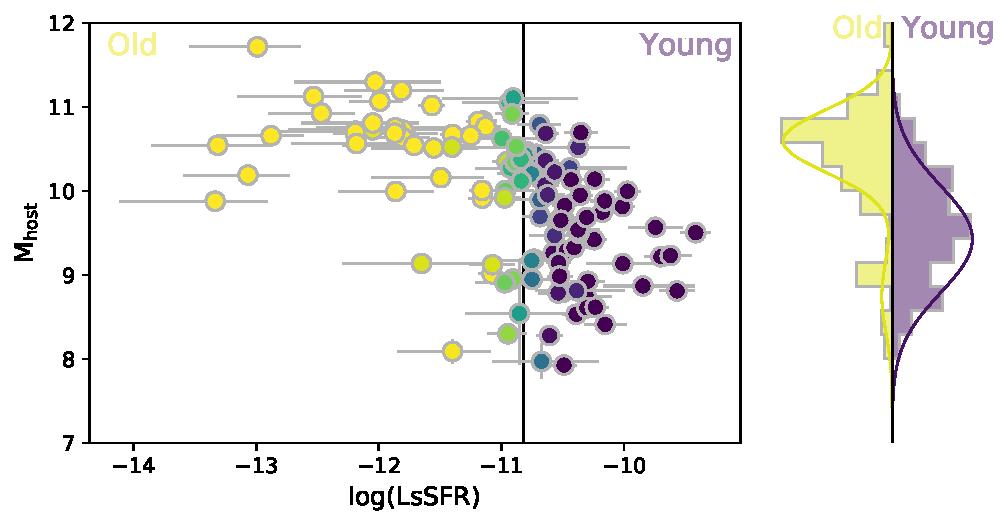
\includegraphics[width=\linewidth]{model_mass_3G3M3S_hist.pdf}
    \caption{\textit{Main}: SED-fitted host mass
        ($M_\mathrm{host}$) as a function of the LsSFR for SNfactory SNe. The color
        corresponds to the probability, $p_y$, for the SNe~Ia to be young, i.e.,
        to have $\log\mathrm{LsSFR} \geq -10.82$ \citep[see][]{rigault2020}.
    \textit{Right}: $p_y$-weighted histogram of the SN masses, as well as the
adjusted model; contributions of the younger and older population are shown
in purple and yellow, respectively.}
    \label{fig:massmodel}
\end{figure}

\begin{table*}
    \centering
    \caption{Best-fit values of the parameters for the mass distribution
    model when applied to the SNfactory dataset only (114 SNe~Ia).}
    \label{tab:modelresults}
    \begin{tabular}{lccccccc}
        \hline\hline
        Sample  & $\mu_\mathrm{y}  $ & $\sigma_\mathrm{y}$
                & $\mu_\mathrm{o,1}$ & $\sigma_\mathrm{o,1}$
                & $\mu_\mathrm{o,2}$ & $\sigma_\mathrm{o,2}$
                & $a$ \\
        \hline
        SNfactory & $ 9.41 \pm ???? $ & $0.62 \pm ????$
                  & $10.60 \pm ???? $ & $0.38 \pm ????$
                  & $ 8.74 \pm ???? $ & $0.43 \pm ????$
                  & $ 0.90 \pm ???? $ \\
        \hline
    \end{tabular}
\end{table*}

\subsection{Input generation}

Then, from a redshift, we can generate a mass and a stretch. This is done with
the \textit{SNprop} Python module (INSERT URL). Given a redshift or lists of
redshift, it takes the expected fraction of young stars using $\delta(z) =
\left( K^{-1}\times \left( 1+z \right)^{-2.8} + 1 \right)^{-1}$ (Fig.
\ref{fig:deltaz} from \cite{rigault2020} then sets a ``young'' or ``old'' flag
by picking a random value between 0 and 1 and comparing it to said fraction. If
the random value is lower, the SN that will be simulated is young. The higher
the $z$, the higher the $\delta(z)$, and thus the lower the probability to flag
it young. Stretch values are then generated with the previous NR21 model
depending whether the progenitor is considered young or old, same for old. We
also include the magnitude shift which we intend to be the underlying reason
behind the mass step.

\begin{figure}[]
    \centering
    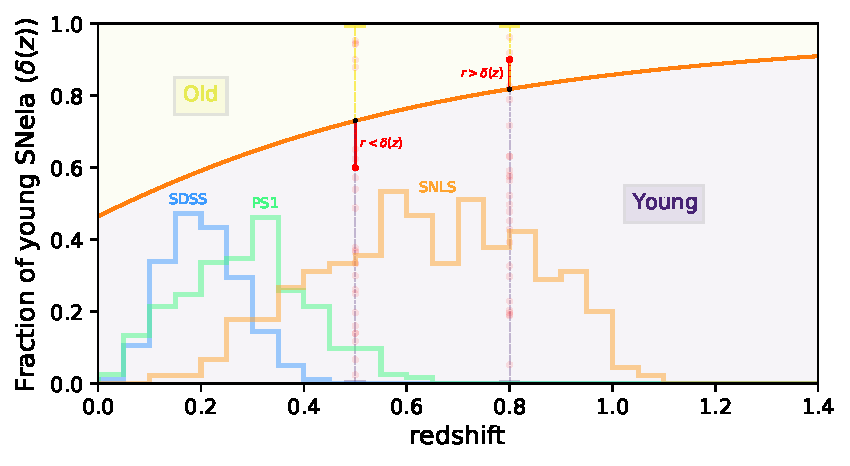
\includegraphics[width=\linewidth]{deltaz_hist_yo-random.pdf}
    \caption{\textit{Orange}: Estimated fraction of young SNe as a function of
        redshift. \textit{Histograms}: Number of SNe in bins of redshift for the
        3 main surveys of the Pantheon sample, not scaled. \textit{Red vertical
        lines}: For each $z$, a random number $a$ between 0 and 1 is picked: if
    it's lower (higher) than $\delta(z)$ at that redshift then the SN will be
young (old), and the distributions of mass and stretch to pick from will follow
this flag.}
    \label{fig:deltaz}
\end{figure}

\subsection{Generating HOSTLIBs}
Generate $z$, take closest $M$ entry in a table of host galaxies (HOSTLIB), then
pick $x_1$, $c$ assuming underlying relationships defined by the BBC team.
Because we want to make these simulations with an evolving underlying
distribution, we have to replace then $x_1$ values by what is estimated by our
previous model. 

\section{SNANA}
What is SNANA doing generally: 3 steps.

Model SN and what will a survey look like: lightcurves
Fitting with SALT.2
Compute distance

In the simulation you take an underlying model of how a SN works and run that
through an obversing lens of a survey to use them like data then fit, and infer
deistances. Basic SNANA. Key is saying what is the definition of a realistic
model? SK16, but no relation with galaxy. P21 or M20 introduced a link between
the two thanks to a HOSTLIB: take a model and turn them into objects. SK16 is
galaxy distribution from which you draw, P21 is a list with the distrubtion
already in it, linking the relationships and $x_1$ and stuff already drawn. But
there's no evolution in it, and we want to do that. Forward model that through.
PREDICTIVE.

SK16: SNe independent galaxies
P21: There is a relationship, we'll try to guess it. Take data bns of mass, and
calculate what the distribtion of stretch is for each. Looks differently in
different bins: as a function of mass they have distribution. Backward models.
N21: our data is independent and we use it to show tht it work on other data at
higher redshift, is predictive.

General, Brodie, us; no lightcurve fitting, and at the end of hostlib section w
simulate antheon

Compare the , x, c distributons we use wih data

Section 3

Having mass isn't constitutive of SNANA, not a requirment, but we use it because
the actual data we compare our simulated data to is described using mass. So we
need a link betwwen LsSFR to mass: high-redshift galaxies only have mass
measurments, not LsSFR. Quote Martin's paper.

given model and observation strategy, what do you see like SIMSURVEY.

SImulation part of SNANA separate from distance.


\section{Results of modeling}
\begin{itemize}
    \item Recreate non-evolving, POPOVIC 21 model;
    \item Test different inputs to reproduce what we want to test.
\end{itemize}

How to check validity of results: SNprop module, copute probability of fit with
a 2D gaussian KDE.

\section{Impact on cosmology}
What we want is not so much $w$ than $\Delta w$ wrt. best current work. We find
x\% and here are the contours.

\section{Discussion}\label{sec:discussion}
We expected to have a higher/lower, and we got that.

\section{Conclusion}\label{sec:ccl}

Should be nice.

\begin{acknowledgements}
    This project has received funding from the European Research Council (ERC)
    under the European Union's Horizon 2020 Research and Innovation program
    (grant agreement no 759194 - USNAC).
    This work was supported in part by the Director, Office of Science, Office
    of High Energy Physics of the U.S. Department of Energy under Contract No.
    DE-AC025CH11231.
    This project is partly financially supported by Région Rhône-Alpes-Auvergne.
\end{acknowledgements}

\end{document}
\bibliographystyle{aa}
\begin{thebibliography}{} 
% A

\bibitem[Abbott et al.(2019)]{descosmopaper2019} Abbott, T.~M.~C., Allam, S.,
Andersen, P., et al.\ 2019, \apjl, 872, L30

\bibitem[Aldering et al.(2002)]{aldering2002} Aldering, G., Adam, G., Antilogus,
P., et al.\ 2002, \procspie, 61

\bibitem[Aldering et al.(2020)]{aldering2020} Aldering, G., Antilogus, P.,
Aragon, C., et al.\ 2020, Research Notes of the American Astronomical Society,
4, 63

\bibitem[Astier et al.(2006)]{astier2006} Astier, P., Guy, J., Regnault, N., et
al.\ 2006, \aap, 447, 31

\bibitem[Aubourg et al.(2008)]{aubourg2008} Aubourg, {\'E}., Tojeiro, R.,
Jimenez, R., et al.\ 2008, \aap, 492, 631 

% B

\bibitem[Bazin et al.(2011)]{bazin2011} Bazin, G., Ruhlmann-Kleider, V.,
Palanque-Delabrouille, N., et al.\ 2011, \aap, 534, A43

\bibitem[Bellm et al.(2019)]{bellm2019} Bellm, E.~C., Kulkarni, S.~R., Graham,
M.~J., et al.\ 2019, \pasp, 131, 018002

\bibitem[Betoule et al.(2014)]{betoule2014} Betoule, M., Kessler, R., Guy, J.,
et al.\ 2014, \aap, 568, A22

\bibitem[Burnham \& Anderson(2004)]{burnham2004} Burnham, K., Anderson, D., \
2004, Sociological Methods \& Research, 33, 2

% C

\bibitem[Campbell et al.(2013)]{campbell2013} Campbell, H., D'Andrea, C.~B.,
Nichol, R.~C., et al.\ 2013, \apj, 763, 88

\bibitem[Childress et al.(2013)]{childress2013} Childress, M., Aldering, G.,
Antilogus, P., et al.\ 2013, \apj, 770, 108

\bibitem[Childress et al.(2014)]{childress2014} Childress, M.~J., Wolf, C., \&
Zahid, H.~J.\ 2014, \mnras, 445, 1898

% D

\bibitem[D'Andrea et al.(2011)]{dandrea2011} D'Andrea, C.~B., Gupta, R.~R.,
Sako, M., et al.\ 2011, \apj, 743, 172

\bibitem[Dilday et al.(2008)]{dilday2008} Dilday, B., Kessler, R., Frieman,
J.~A., et al.\ 2008, \apj, 682, 262

% E
% F

\bibitem[Feeney et al.(2019)]{feeney2019} Feeney, S.~M., Peiris, H.~V.,
Williamson, A.~R., et al.\ 2019, \prl, 122, 061105

\bibitem[Freedman et al.(2019)]{freedman2019} Freedman, W.~L., Madore, B.~F.,
Hatt, D., et al.\ 2019, \apj, 882, 34

\bibitem[Freedman et al.(2020)]{freedman2020} Freedman, W.~L., Madore, B.~F.,
Hoyt, T., et al.\ 2020, \apj, 891, 57. doi:10.3847/1538-4357/ab7339

\bibitem[Frieman et al.(2008)]{frieman2008} Frieman, J.~A., Bassett, B., Becker,
A., et al.\ 2008, \aj, 135, 338

% G

\bibitem[Graham et al.(2019)]{graham2019} Graham, M.~J., Kulkarni, S.~R., Bellm,
E.~C., et al.\ 2019, \pasp, 131, 078001

\bibitem[Gupta et al.(2011)]{gupta2011} Gupta, R.~R., D'Andrea, C.~B., Sako, M.,
et al.\ 2011, \apj, 740, 92

\bibitem[Guy et al.(2007)]{guy2007} Guy, J., Astier, P., Baumont, S., et al.\
2007, \aap, 466, 11

% H

\bibitem[Hamuy et al.(1996)]{hamuy1996} Hamuy, M., Phillips, M.~M., Suntzeff,
N.~B., et al.\ 1996, \aj, 112, 2391

\bibitem[Hamuy et al.(2000)]{hamuy2000} Hamuy, M., Trager, S.~C., Pinto, P.~A.,
et al.\ 2000, \aj, 120, 1479

\bibitem[Hinton et al.(2019)]{hinton2019} Hinton, S.~R., Davis, T.~M., Kim,
A.~G., et al.\ 2019, \apj, 876, 15

\bibitem[Howell et al.(2007)]{howell2007} Howell, D.~A., Sullivan, M., Conley,
A., et al.\ 2007, \apjl, 667, L37

% I

\bibitem[Ivezi{\'c} et al.(2019)]{lsstpaper} Ivezi{\'c}, {\v{Z}}., Kahn, S.~M.,
Tyson, J.~A., et al.\ 2019, \apj, 873, 111

% J

\bibitem[Jones et al.(2015)]{jones2015} Jones, D.~O., Riess, A.~G., \& Scolnic,
D.~M.\ 2015, \apj, 812, 3 1

\bibitem[Jones et al.(2019)]{jones2019} Jones, D.~O., Scolnic, D.~M., Foley,
R.~J., et al.\ 2019, \apj, 881, 19

% K

\bibitem[Kelly et al.(2010)]{kelly2010} Kelly, P.~L., Hicken, M., Burke, D.~L.,
et al.\ 2010, \apj, 715, 743

\bibitem[Kessler et al.(2009)]{kessler2009} Kessler, R., Becker, A.~C., Cinabro,
D., et al.\ 2009, \apjs, 185, 32

\bibitem[Kessler et al.(2009)]{SNANA} Kessler, R., Bernstein, J.~P., Cinabro,
D., et al.\ 2009, \pasp, 121, 1028

\bibitem[Kessler \& Scolnic(2017)]{kessler2017} Kessler, R., \& Scolnic, D.\
2017, \apj, 836, 56

\bibitem[Kim et al.(2018)]{kim18} Kim, Y.-L., Smith, M., Sullivan, M., et al.\
2018, \apj, 854, 24

\bibitem[Kim et al.(2019)]{kim19} Kim, Y.-L., Kang, Y., \& Lee, Y.-W.\ 2019,
Journal of Korean Astronomical Society, 52, 181

\bibitem[Knox \& Millea(2020)]{knox2019} Knox, L. \& Millea, M.\ 2020, \prd,
101, 043533. doi:10.1103/PhysRevD.101.043533

% L

\bibitem[Lampeitl et al.(2010)]{lampeitl2010} Lampeitl, H., Smith, M., Nichol,
R.~C., et al.\ 2010, \apj, 722, 566

% M

\bibitem[Mannucci et al.(2005)]{mannucci2005} Mannucci, F., Della Valle, M.,
Panagia, N., et al.\ 2005, \aap, 433, 807 

\bibitem[Mannucci et al.(2006)]{mannucci2006} Mannucci, F., Della Valle, M., \&
Panagia, N.\ 2006, \mnras, 370, 773 

\bibitem[Maoz et al.(2014)]{maozmannucci2014} Maoz, D., Mannucci, F., \&
Nelemans, G.\ 2014, \araa, 52, 107 


% N

\bibitem[Neill et al.(2006)]{neill2006} Neill, J.~D., Sullivan, M., Balam, D.,
et al.\ 2006, \aj, 132, 1126

\bibitem[Neill et al.(2009)]{neill2009} Neill, J.~D., Sullivan, M., Howell,
D.~A., et al.\ 2009, \apj, 707, 1449

\bibitem[Nordin et al.(2018)]{nordin2018} Nordin, J., Aldering, G., Antilogus,
P., et al.\ 2018, \aap, 614, A71

% O
% P

\bibitem[Pan et al.(2014)]{pan2014} Pan, Y.-C., Sullivan, M., Maguire, K., et
al.\ 2014, \mnras, 438, 1391

\bibitem[Perlmutter et al.(1999)]{perlmutter1999} Perlmutter, S., Aldering, G.,
Goldhaber, G., et al.\ 1999, \apj, 517, 565

\bibitem[Perrett et al.(2010)]{perrett2010} Perrett, K., Balam, D., Sullivan,
M., et al.\ 2010, \aj, 140, 518

\bibitem[Phillips(1993)]{phillips1993} Phillips, M.~M.\ 1993, \apjl, 413, L105

\bibitem[Planck Collaboration et al.(2020)]{planck2018} Planck
Collaboration, Aghanim, N., Akrami, Y., et al.\ 2020, \aap, 641, A6.
doi:10.1051/0004-6361/201833910

% Q
% R

\bibitem[Reid et al.(2019)]{reid2019} Reid, M.~J., Pesce, D.~W., \& Riess,
A.~G.\ 2019, \apjl, 886, L27. doi:10.3847/2041-8213/ab552d

\bibitem[Rest et al.(2014)]{rest2014} Rest, A., Scolnic, D., Foley, R.~J., et
al.\ 2014, \apj, 795, 44

\bibitem[Riess et al.(1998)]{riess1998} Riess, A.~G., Filippenko, A.~V.,
Challis, P., et al.\ 1998, \aj, 116, 1009

\bibitem[Riess et al.(2009)]{riess2009} Riess, A.~G., Macri, L., Casertano, S.,
et al.\ 2009, \apj, 699, 539

\bibitem[Riess et al.(2016)]{riess2016} Riess, A.~G., Macri, L.~M., Hoffmann,
S.~L., et al.\ 2016, \apj, 826, 56

\bibitem[Riess et al.(2018)]{riess2018} Riess, A.~G., Casertano, S., Yuan, W.,
et al.\ 2018, \apj, 861, 126

\bibitem[Riess et al.(2019)]{riess2019} Riess, A.~G., Casertano, S., Yuan, W.,
et al.\ 2019, \apj, 876, 85

\bibitem[{Rigault et al.(2013)}]{rigault2013} Rigault, M., Copin, Y.,
Aldering, G., {et~al.} 2013, \aap, 560, A66

\bibitem[Rigault et al.(2015)]{rigault2015} Rigault, M., Aldering, G., Kowalski,
M., et al.\ 2015, \apj, 802, 20

\bibitem[Rigault et al.(2020)]{rigault2020} Rigault, M., Brinnel, V., Aldering,
G., et al.\ 2020, \aap, 644, A176

\bibitem[Rodney et al.(2014)]{rodney2014} Rodney, S.~A., Riess, A.~G., Strolger,
L.-G., et al.\ 2014, \aj, 148, 13 
  
\bibitem[Roman et al.(2018)]{roman2018} Roman, M., Hardin, D., Betoule, M., et
al.\ 2018, \aap, 615, A68

\bibitem[Rose et al.(2019)]{rose2019} Rose, B.~M., Garnavich, P.~M., \& Berg,
M.~A.\ 2019, \apj, 874, 32

\bibitem[Rubin et al.(2015)]{rubin2015} Rubin, D., Aldering, G., Barbary, K., et
al.\ 2015, \apj, 813, 137

\bibitem[Rubin \& Hayden(2016)]{rubin2016} Rubin, D., \& Hayden, B.\ 2016,
\apjl, 833, L30

% S

\bibitem[Sako et al.(2008)]{sako,2008} Sako, M., Bassett, B., Becker, A., et al.\
2008, \aj, 135, 348

\bibitem[Scannapieco \& Bildsten(2005)]{scannapieco,2005} Scannapieco, E., \&
Bildsten, L.\ 2005, \apjl, 629, L85 

\bibitem[Scolnic et al.(2014)]{scolnic2014} Scolnic, D., Rest, A., Riess, A., et
al.\ 2014, \apj, 795, 45

\bibitem[Scolnic \& Kessler(2016)]{scolnic2016} Scolnic, D., \& Kessler, R.\
2016, \apjl, 822, L35

\bibitem[Scolnic et al.(2018)]{scolnic2018a} Scolnic, D.~M., Jones, D.~O., Rest,
A., et al.\ 2018a, \apj, 859, 101

\bibitem[Scolnic et al.(2019)]{scolnicastro,2020} Scolnic, D., Perlmutter, S.,
Aldering, G., et al.\ 2019, Astro,2020: Decadal Survey on Astronomy and
Astrophysics, 2020, 270

\bibitem[Shariff et al.(2016)]{shariff2016} Shariff, H., Jiao, X., Trotta, R.,
et al.\ 2016, \apj, 827, 1

\bibitem[Smith et al.(2012)]{smith2012} Smith, M., Nichol, R.~C., Dilday, B., et
al.\ 2012, \apj, 755, 61

\bibitem[Smith et al.(2020)]{smith2020} Smith, M., Sullivan, M., Wiseman, P., et
al.\ 2020, \mnras, 494, 4426

\bibitem[Strolger et al.(2004)]{strolger04} Strolger, L.-G., Riess, A.~G., et
al.\ 2004, \apj, 613, 200

\bibitem[Sullivan et al.(2006)]{sullivan2006} Sullivan, M., Le Borgne, D.,
Pritchet, C.~J., et al.\ 2006, \apj, 648, 868 

\bibitem[Sullivan et al.(2010)]{sullivan2010} Sullivan, M., Conley, A., Howell,
D.~A., et al.\ 2010, \mnras, 406, 782

% T

\bibitem[Tasca et al.(2015)]{tasca2015} Tasca, L.~A.~M., Le F{\`e}vre, O.,
Hathi, N.~P., et al.\ 2015, \aap, 581, A54

% U 
% V
% W

\bibitem[Wiseman et al.(2020)]{wiseman2020} Wiseman, P., Smith, M., Childress,
M., et al.\ 2020, \mnras, 495, 4040. doi:10.1093/mnras/staa1302

\bibitem[Wong et al.(2020)]{wong2019} Wong, K.~C., Suyu, S.~H., Chen, G.~C.-F.,
et al.\ 2020, \mnras, 498, 1420. doi:10.1093/mnras/stz3094

% X
% Y
% Z
\end{thebibliography}
